\documentclass{article}

\usepackage[a4paper, margin=1in]{geometry}
\usepackage{amsmath}
\usepackage{bm}
\usepackage[usenames, dvipsnames]{xcolor}
\usepackage{url}
\usepackage[title]{appendix}

\usepackage[dvipdfmx]{graphicx}
\graphicspath{ {./images/} }

\usepackage{listings}
\lstset{
  frame=lines,
  label={lst:code_direct},
  basicstyle=\footnotesize,
  numbers=left
}

\title{Graph Based SLAM}
\date{}
\author{}

\begin{document}

\maketitle

\section{What is Graph Based SLAM?}

Graph Based SALM is one of the offline SLAM method, which means correcting whole historical robot trajectory and landmarks position using all observation data.
Considering a robot pose at time $t_i$ as a node and a vector between 2 nodes (between 2 robot poses at time $t_i$ and $t_j$) as an edge, Graph Based SLAM will try to find the best estimated robot and landmarks poses that minimize a cost function.
The cost function contains all errors between a motion edge and a corresponding observation edge.

\begin{figure}[h!]
  \centering
  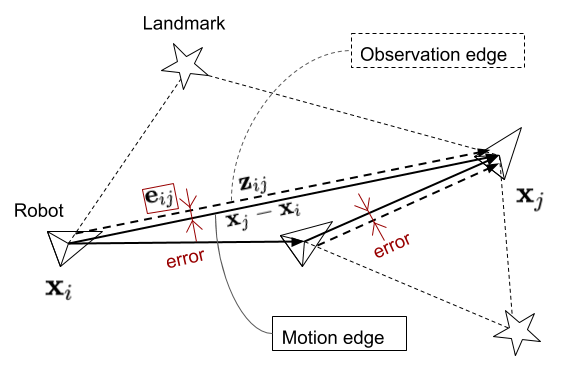
\includegraphics[width=0.8\textwidth]{1-1_error_between_edges.png}
\end{figure}

The error $\bm{e}_{ij}$ between a motion edge and an observation edge in different pose $i$ and $j$ is;

\[
\bm{e}_{ij}(\bm{x}_i, \bm{x}_j) = (\bm{x}_j - \bm{x}_i) - \bm{z}_{ij}
\]

where $\bm{x}_i$ and $\bm{x}_j$ are the robot poses in time step $i$ and $j$ respectively, and $\bm{z}_{ij}$ is the edge obtained by observing a same landmark in pose $i$ and $j$.
Thus, the cost function $F(\bm{x}_{0:t})$ can be expressed as;

\[
F(\bm{x}_{0:t}) = \sum_{i,j} \bm{e}_{ij}(\bm{x}_i, \bm{x}_j)^{\mathrm{T}} \Omega_{ij} \bm{e}_{ij}(\bm{x}_i, \bm{x}_j)
\]

that is the sum of square errors $\bm{e}_{ij}^{\mathrm{T}} \bm{e}_{ij}$ weighted by information matrix $\Omega_{ij}$, which expresses accuracy of the edge (Mahalanobis distance).
The aim of Graph Based SLAM is to find the robot and landmarks poses that minimize this cost function.

\newpage

\section{Definitions}

Defines some coordinates and variables used in this document.

\subsection{Coordinate}

There are 2 robot poses and 1 landmark on $Absolute$ coordinate.
Each robot pose has own $Vehicle$ coordinate, the X axis is the heading direction and Y axis is the left hand of the robot.
Assumes that every landmark has own angle, although the absolute value of the landmark's angle is not so important (to be discussed later).

\begin{figure}[h!]
  \centering
  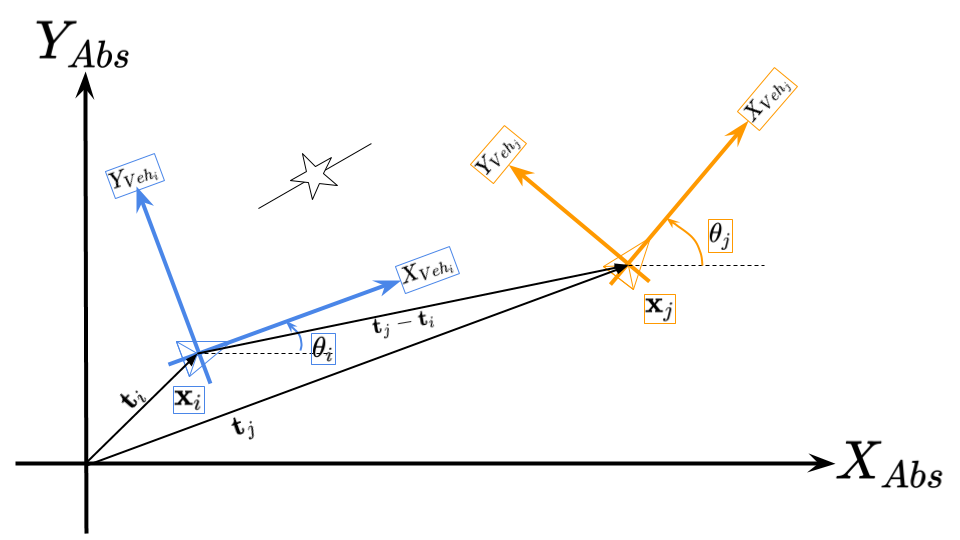
\includegraphics[width=\textwidth]{2-1_coordinate.png}
\end{figure}

\subsection{Robot position vector: $\bm{t}_i$}

It contains robot position $x_i$ and $y_i$ on $Absolute$ coordinate.

\[
\bm{t}_i =
\left(
  \begin{array}{c}
    x_i \\
    y_i \\
  \end{array}
\right)
\]

\subsection{Robot state vector: $\bm{x}_i$}

However, the robot pose has another parameter, which is yaw angle $\theta_i$ on $Absolute$ coordinate.

\[
\bm{x}_i =
\left(
  \begin{array}{c}
    \bm{t}_i \\
    \theta_i \\
  \end{array}
\right)
=
\left(
  \begin{array}{c}
    x_i \\
    y_i \\
    \theta_i \\
  \end{array}
\right)
\]

\newpage

\subsection{Rotation matrix: $R_i$}

This matrix rotates the coordinate clockwise.
In particular, $R_i$ converts $Vehicle_i$ coordinate into the $Absolute$ coordinate.

\[
R_i =
\left(
  \begin{array}{ccc}
    cos\theta_i & -sin\theta_i \\
    sin\theta_i &  cos\theta_i \\
  \end{array}
\right)
\]

\begin{figure}[h!]
  \centering
  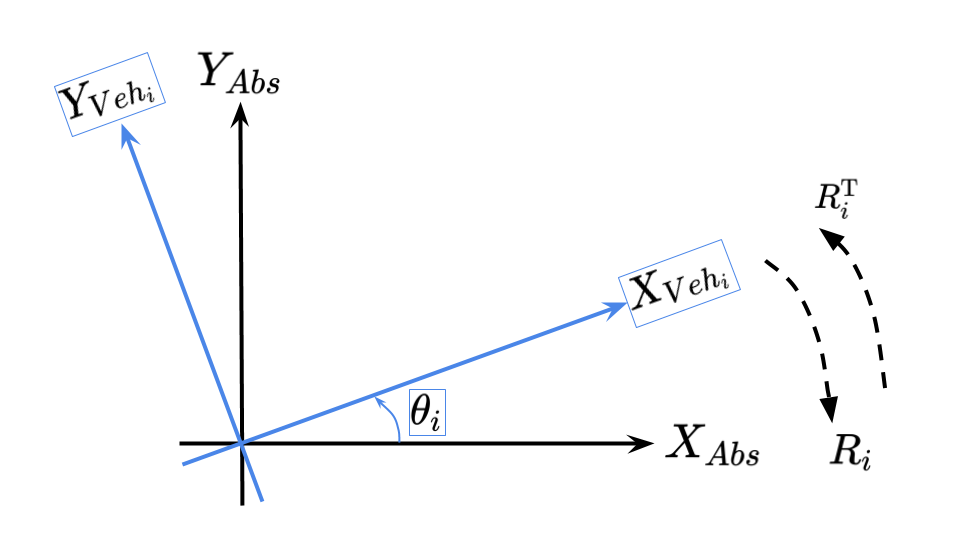
\includegraphics[width=0.6\textwidth]{2-2_rotation_matrix.png}
\end{figure}

\subsection{Pose representation matrix: $X_i$}

One of the way to represent the robot pose is transformation matrix, but there are a number of alternatives.
In this document, the pose representation matrix consists of rotation matrix $R_i$ and robot position vector $t_i$.

\[
X_i =
\left(
  \begin{array}{ccc}
    R_i & \bm{t}_i \\
     00 &          1 \\
  \end{array}
\right)
=
\left(
  \begin{array}{ccc}
    cos\theta_i & -sin\theta_i & x_i \\
    sin\theta_i &  cos\theta_i & y_i \\
              0 &            0 &   1 \\
  \end{array}
\right)
\]

\begin{figure}[h!]
  \centering
  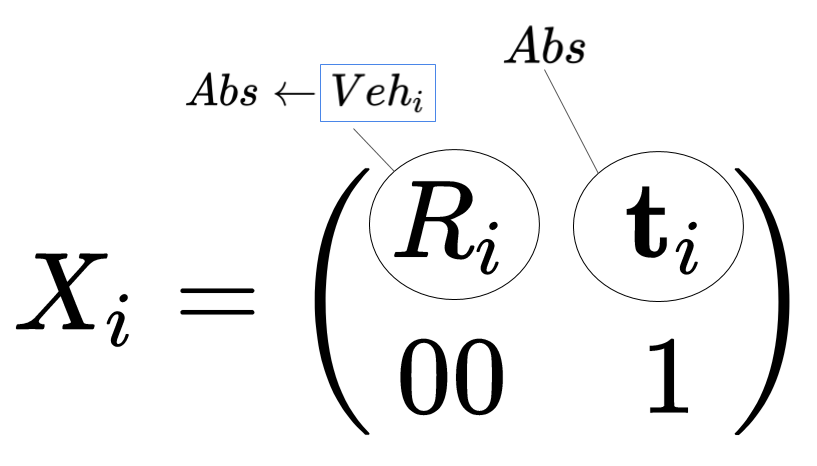
\includegraphics[width=0.4\textwidth]{2-3_pose_representation_matrix.png}
\end{figure}

The inverse of the pose representation matrix has power to convert the origin from $Absolute$ coordinate into own coordinate.
In particular, $X_i^{\mathrm{T}}$ converts the origin from $Absolute$ coordinate into $Vehicle_i$ coordinate.

\[
X_i^{-1} =
\left(
  \begin{array}{ccc}
    R_i^{\mathrm{T}} & -R_i^{\mathrm{T}}\bm{t}_i \\
                  00 &                           1 \\
  \end{array}
\right)
\]

\begin{figure}[h!]
  \centering
  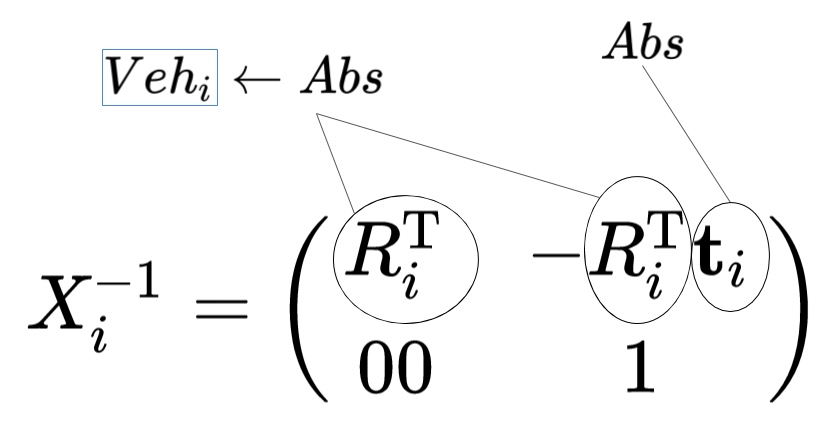
\includegraphics[width=0.4\textwidth]{2-4_pose_representation_matrix_inverse.png}
\end{figure}

\newpage

\subsection{Sensor model}

The sensor on the robot observes two information, the distance $d$ and the angle $\varphi$ from the robot to a landmark.
When the robot in a pose $i$ and $j$ observe a same landmark, the robot can calculate the difference of the landmark angle $\psi_i - \psi_j$ from each view by using computer vision or something, although the robot doesn't know the absolute values of $\psi_i$ and $\psi_j$ (the robot only can know the relative value).
And $\theta_{ij}$ in the observation representation $Z_{ij}$ denotes this relative value of the landmark angle $\psi_i - \psi_j$ from each view.

\begin{figure}[h!]
  \centering
  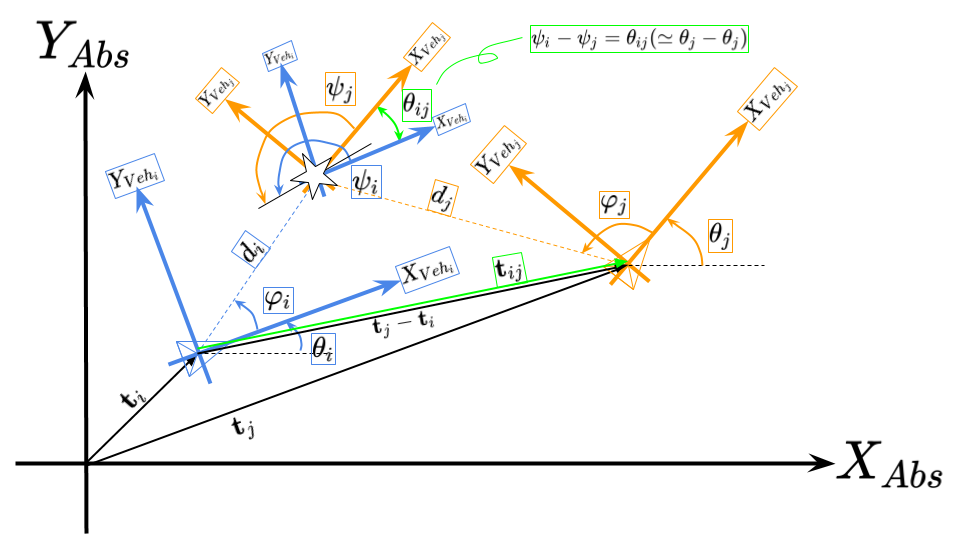
\includegraphics[width=\textwidth]{2-7_sensor_model.png}
\end{figure}

\subsection{Observation representation matrix: $Z_{ij}$}

If the robot in different poses observe a same landmark, then the relative pose of the robot between these poses can be calculated from the view of the landmark.
Assumes that the robot in a pose $i$ and $j$ observe a same landmark, the observation representation $Z_{ij}$ will be,

\[
Z_{ij} =
\left(
  \begin{array}{ccc}
    R_{ij} & \bm{t}_{ij} \\
       00 &              1 \\
  \end{array}
\right)
=
\left(
  \begin{array}{ccc}
    cos\theta_{ij} & -sin\theta_{ij} & x_{ij} \\
    sin\theta_{ij} &  cos\theta_{ij} & y_{ij} \\
                0 &                0 &      1 \\
  \end{array}
\right)
\]

\begin{figure}[h!]
  \centering
  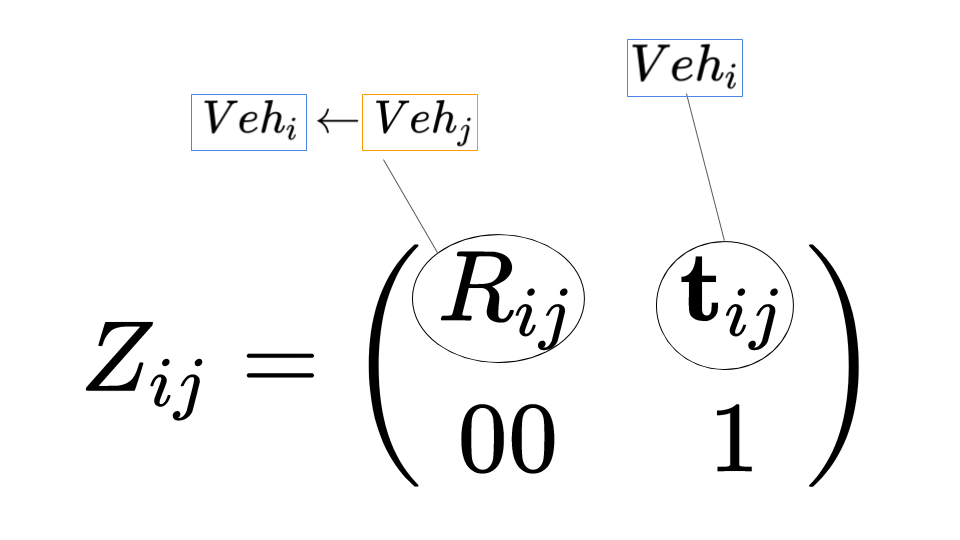
\includegraphics[width=0.4\textwidth]{2-5_observation_representation_matrix.png}
  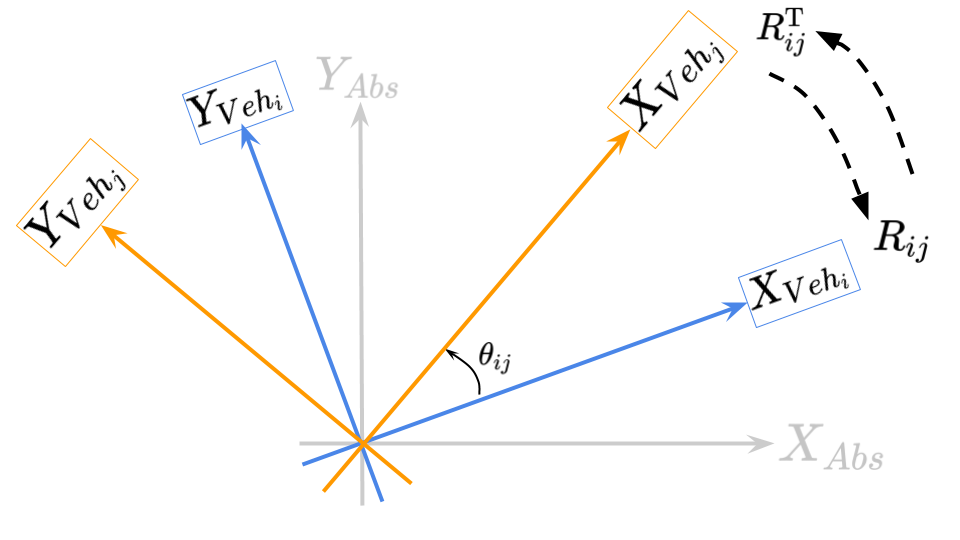
\includegraphics[width=0.5\textwidth]{2-6_rotation_matrix.png}
\end{figure}

The origin of the observation representation $Z_{ij}$ is on $Vehicle_i$ coordinate, thus $\bm{t}_{ij}$ means the distance and $\theta_{ij}$ means the angle from $Vehicle_i$ coordinate to $Vehicle_j$ coordinate.

\newpage

\section{Optimization} \label{optimization}

The cost function calculated by errors between edges can be optimized using a least square method such as the Gauss-Newton algorithm.

\subsection{Error and Cost function}

The $\bm{t}_{ij}$ and $\theta_{ij} (= \psi_i - \psi_j)$ in the observation representation $Z_{ij}$ should be equal to the difference of the position $\bm{t}_j - \bm{t}_i$ and the angle $\theta_j - \theta_i$ respectively in an ideal environment.
However in the real world, these values are different due to sensor error.

\[
\bm{e}_{ij}(\bm{x}_i, \bm{x}_j) = (\bm{x}_j - \bm{x}_i) - \bm{z}_{ij}
\]

The error function $\bm{e}_{ij}(\bm{x}_i, \bm{x}_j)$ can be expressed by using the pose representation matrix $X_i$, $X_j$ and the observation representation matrix $Z_{ij}$ introduced in the previous section.
First, the motion edge between poses in time step $i$ and $j$ is calculated by multiplying the inverse of $i$ th pose representation $X_i^{-1}$ to $j$ th pose representation $X_j$;

\[
\begin{align}
X_i^{-1} X_j &=
\left(
  \begin{array}{cc}
    R_i^{\mathrm{T}} & -R_i^{\mathrm{T}}\bm{t}_i \\
                  00 &                           1 \\
  \end{array}
\right)
\left(
  \begin{array}{cc}
    R_j & \bm{t}_j \\
     00 &          1 \\
  \end{array}
\right) \\ &=
\left(
  \begin{array}{cc}
    R_i^{\mathrm{T}}R_j & R_i^{\mathrm{T}}(\bm{t}_j-\bm{t}_i) \\
                     00 &                                       1 \\
  \end{array}
\right)
\end{align}
\]

\begin{figure}[h!]
  \centering
  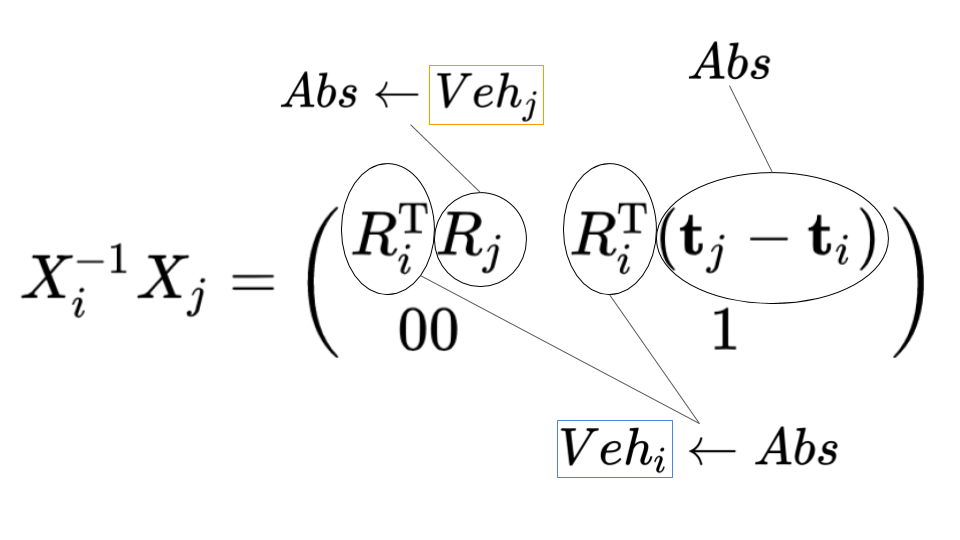
\includegraphics[width=0.5\textwidth]{3-1_difference_between_nodes.png}
\end{figure}

Then, the error $\bm{e}_{ij}(\bm{x}_i, \bm{x}_j)$ between the motion edge and the corresponding observation edge is obtained by multiplying the inverse of the observation representation $Z_{ij}^{-1}$;

\[
\begin{align}
Z_{ij}^{-1} (X_i^{-1} X_j) &=
\left(
  \begin{array}{cc}
    R_{ij}^{\mathrm{T}} & -R_{ij}^{\mathrm{T}}\bm{t}_{ij} \\
                     00 &                                 1 \\
  \end{array}
\right)
\left(
  \begin{array}{cc}
    R_i^{\mathrm{T}}R_j & R_i^{\mathrm{T}}(\bm{t}_j-\bm{t}_i) \\
                     00 &                                       1 \\
  \end{array}
\right) \\ &=
\left(
  \begin{array}{cc}
    R_{ij}^{\mathrm{T}}R_i^{\mathrm{T}}R_j & R_{ij}^{\mathrm{T}}\{R_i^{\mathrm{T}}(\bm{t}_j-\bm{t}_i)-\bm{t}_{ij}\} \\
                                        00 &                                                                            1 \\
  \end{array}
\right)
\end{align}
\]

\begin{figure}[h!]
  \centering
  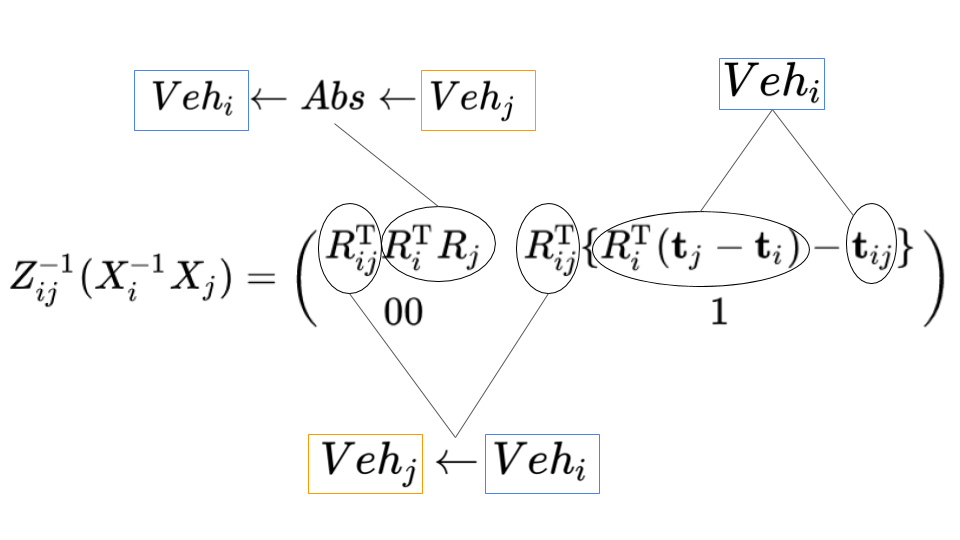
\includegraphics[width=0.6\textwidth]{3-2_error_between_edges.png}
\end{figure}

\newpage

The error function $\bm{e}_{ij}(\bm{x}_i, \bm{x}_j)$ consists of the translation elements $R_{ij}^{\mathrm{T}}\{R_i^{\mathrm{T}}(\bm{t}_j-\bm{t}_i)-\bm{t}_{ij}\}$ and the (angle of the) rotation elements $R_{ij}^{\mathrm{T}}R_i^{\mathrm{T}}R_j$ of this matrix $Z_{ij}^{-1} (X_i^{-1} X_j)$;

\[
\begin{align}
\bm{e}_{ij}(\bm{x}_i, \bm{x}_j) &=
\left(
  \begin{array}{cc}
    R_{ij}^{\mathrm{T}}\{R_i^{\mathrm{T}}(\bm{t}_j-\bm{t}_i)-\bm{t}_{ij}\} \\
                                   angle(R_{ij}^{\mathrm{T}}R_i^{\mathrm{T}}R_j) \\
  \end{array}
\right) \\ &=
\left(
  \begin{array}{cc}
    R_{ij}^{\mathrm{T}}\{R_i^{\mathrm{T}}(\bm{t}_j-\bm{t}_i)-\bm{t}_{ij}\} \\
                                             (\theta_j - \theta_i) - \theta_{ij} \\
  \end{array}
\right)
\end{align}
\]

The objective of Graph Based SLAM is to reduce these errors --- between \textit{Motion model} and \textit{Observation model} --- by using weighted square errors (Mahalanobis distance) and a least squares method (the Gauss-Newton algorithm) with a sparse graph structure.
The cost function is the sum of the weighted square errors $\bm{e}_{ij}(\bm{x}_i, \bm{x}_j)$ across all observation data;

\[
\begin{align}
F(\bm{x}_{0:t}) &=
\sum_{i,j} \bm{e}_{ij}(\bm{x}_i, \bm{x}_j)^{\mathrm{T}} \Omega_{ij} \bm{e}_{ij}(\bm{x}_i, \bm{x}_j) \\ &=
\bm{e}_{0:t}(\bm{x}_{0:t})^{\mathrm{T}} \Omega_{0:t} \bm{e}_{0:t}(\bm{x}_{0:t})
\end{align}
\]

\subsection{Linearization}

The Gauss-Newton algorithm is used to minimize this const function.
The idea is to approximate the error function by its 1st order Taylor expansion around the current initial guess $\bm{x}_{0:t}$.

\[
\begin{align}
F(\bm{x}_{0:t} + \Delta\bm{x}_{0:t}) &=
\bm{e}_{0:t}(\bm{x}_{0:t} + \Delta\bm{x}_{0:t})^{\mathrm{T}}
  \Omega_{0:t}
    \bm{e}_{0:t}(\bm{x}_{0:t} + \Delta\bm{x}_{0:t}) \\ &\simeq
(\bm{e}_{0:t}(\bm{x}_{0:t}) + J_{0:t}\Delta\bm{x}_{0:t})^{\mathrm{T}}
  \Omega_{0:t}
    (\bm{e}_{0:t}(\bm{x}_{0:t}) + J_{0:t}\Delta\bm{x}_{0:t}) \\ &=
\{\bm{e}_{0:t}(\bm{x}_{0:t})^{\mathrm{T}} + (J_{0:t}\Delta\bm{x}_{0:t})^{\mathrm{T}}\}
  \Omega_{0:t}
    (\bm{e}_{0:t}(\bm{x}_{0:t}) + J_{0:t}\Delta\bm{x}_{0:t}) \\ &=
\bm{e}_{0:t}(\bm{x}_{0:t})^{\mathrm{T}} \Omega_{0:t} \bm{e}_{0:t}(\bm{x}_{0:t})
  + (J_{0:t}\Delta\bm{x}_{0:t})^{\mathrm{T}} \Omega_{0:t} \bm{e}_{0:t}(\bm{x}_{0:t}) \\
    &\qquad + \bm{e}_{0:t}(\bm{x}_{0:t})^{\mathrm{T}} \Omega_{0:t} (J_{0:t}\Delta\bm{x}_{0:t})
      + (J_{0:t}\Delta\bm{x}_{0:t})^{\mathrm{T}} \Omega_{0:t} (J_{0:t}\Delta\bm{x}_{0:t}) \\ &=
F(\bm{x}_{0:t})
  + \{(\Omega_{0:t}\bm{e}_{0:t}(\bm{x}_{0:t}))^{\mathrm{T}} (J_{0:t}\Delta\bm{x}_{0:t})\}^{\mathrm{T}}
    + \bm{e}_{0:t}(\bm{x}_{0:t})^{\mathrm{T}} \Omega_{0:t} J_{0:t}\Delta\bm{x}_{0:t}
      + \Delta\bm{x}_{0:t}^{\mathrm{T}}J_{0:t}^{\mathrm{T}} \Omega_{0:t} J_{0:t}\Delta\bm{x}_{0:t}
\end{align}
\]

Since $\Omega_{0:t}$ is a symmetric matrix, and $\bm{e}_{0:t}(\bm{x}_{0:t})^{\mathrm{T}} \Omega_{0:t} J_{0:t}\Delta\bm{x}_{0:t}$ is a scalar,

\[
\begin{align}
F(\bm{x}_{0:t} + \Delta\bm{x}_{0:t}) &\simeq
F(\bm{x}_{0:t})
  + (\bm{e}_{0:t}(\bm{x}_{0:t})^{\mathrm{T}} \Omega_{0:t} J_{0:t}\Delta\bm{x}_{0:t})^{\mathrm{T}}
    + \bm{e}_{0:t}(\bm{x}_{0:t})^{\mathrm{T}} \Omega_{0:t} J_{0:t}\Delta\bm{x}_{0:t}
      + \Delta\bm{x}_{0:t}^{\mathrm{T}}J_{0:t}^{\mathrm{T}} \Omega_{0:t} J_{0:t}\Delta\bm{x}_{0:t} \\ &=
F(\bm{x}_{0:t})
  + 2\bm{e}_{0:t}(\bm{x}_{0:t})^{\mathrm{T}} \Omega_{0:t} J_{0:t}\Delta\bm{x}_{0:t}
    + \Delta\bm{x}_{0:t}^{\mathrm{T}}J_{0:t}^{\mathrm{T}} \Omega_{0:t} J_{0:t}\Delta\bm{x}_{0:t} \\ &=
F(\bm{x}_{0:t})
  + 2\bm{b}_{0:t}^{\mathrm{T}} \Delta\bm{x}_{0:t}
    + \Delta\bm{x}_{0:t}^{\mathrm{T}} H_{0:t} \Delta\bm{x}_{0:t}
\end{align}
\]

where

\[
\bm{b}_{0:t} = J_{0:t}^{\mathrm{T}} \Omega_{0:t} \bm{e}_{0:t}(\bm{x}_{0:t}), \quad H_{0:t} = J_{0:t}^{\mathrm{T}} \Omega_{0:t} J_{0:t}
\]

\subsection{Solve and Update} \label{solveandupdate}

Regards $\bm{x}_{0:t}$ as a constant and ${\Delta\bm{x}}_{0:t}$ is a variable, the ${\Delta\bm{x}}_{0:t}$ which decreases the cost function $F(\bm{x}_{0:t} + \Delta\bm{x}_{0:t})$ most can be derived by differentiating $F(\bm{x}_{0:t} + \Delta\bm{x}_{0:t})$ with respect to ${\Delta\bm{x}}_{0:t}$ and set the differential as zero.

\[
\frac{\partial F(\bm{x}_{0:t} + \Delta\bm{x}_{0:t})}{\partial \Delta\bm{x}_{0:t}} \simeq
2\bm{b}_{0:t} + (H_{0:t} + H_{0:t}^{\mathrm{T}})\Delta\bm{x}_{0:t} =
0
\]

Since $H_{0:t}$ is a symmetric matrix as well (because $\Omega_{0:t}$ is symmetric),

\[
\begin{align}
2\bm{b}_{0:t} + 2H_{0:t}\Delta\bm{x}_{0:t} &= 0 \\
\Delta\bm{x}_{0:t} &= -H_{0:t}^{-1} \bm{b}_{0:t}
\end{align}
\]

The estimated robot poses can be obtained by adding this increments $\Delta\bm{x}_{0:t}$ to the initial guess $\bm{x}_{0:t}$.

\[
\bm{x}_{0:t}' = \bm{x}_{0:t} + \Delta\bm{x}_{0:t}
\]

Finally, recalculates $H_{0:t}$ and $\bm{b}_{0:t}$, and \textbf{iterates} with the previous result until it is converged.

\newpage

\subsection{Information matrix of the system}

Every edge contributes to the system with an addend term.
To calculate the addend term in each edge, $H_{ij}$ and $\bm{b}_{ij}$, separates the Jacobian matrix $J_{ij}$ of the error function $\bm{e}_{ij}(\bm{x}_i, \bm{x}_j)$ into 2 parts, one is about a robot pose $\bm{x}_i$ in pose $i$ and the other one is about a robot pose $\bm{x}_j$ in pose $j$ since the error function depends only on these 2 nodes.

\[
J_{ij} =
\frac{\partial \bm{e}_{ij}(\bm{x}_i, \bm{x}_j)}{\partial (\bm{x}_i,\bm{x}_j)} =
\left(
  \begin{array}{cccccc}
    \frac{\partial e_{ij_x}}{\partial x_i} & \frac{\partial e_{ij_x}}{\partial y_i} & \frac{\partial e_{ij_x}}{\partial \theta_i} & \frac{\partial e_{ij_x}}{\partial x_j} & \frac{\partial e_{ij_x}}{\partial y_j} & \frac{\partial e_{ij_x}}{\partial \theta_j} \\
    \frac{\partial e_{ij_y}}{\partial x_i} & \frac{\partial e_{ij_y}}{\partial y_i} & \frac{\partial e_{ij_y}}{\partial \theta_i} & \frac{\partial e_{ij_y}}{\partial x_j} & \frac{\partial e_{ij_y}}{\partial y_j} & \frac{\partial e_{ij_y}}{\partial \theta_j} \\
    \frac{\partial e_{ij_\theta}}{\partial x_i} & \frac{\partial e_{ij_\theta}}{\partial y_i} & \frac{\partial e_{ij_\theta}}{\partial \theta_i} & \frac{\partial e_{ij_\theta}}{\partial x_j} & \frac{\partial e_{ij_\theta}}{\partial y_j} & \frac{\partial e_{ij_\theta}}{\partial \theta_j} \\
  \end{array}
\right) =
\left(
  \begin{array}{cc}
    A_{ij} & B_{ij} \\
  \end{array}
\right)
\]

where $A_{ij}$ and $B_{ij}$ are the derivatives of the error function $\bm{e}_{ij}(\bm{x}_i, \bm{x}_j)$ with respect to $\bm{x}_i$ and $\bm{x}_j$.

\[
\begin{align}
A_{ij} &=
\left(
  \begin{array}{ccc}
    \frac{\partial e_{ij_x}}{\partial x_i} & \frac{\partial e_{ij_x}}{\partial y_i} & \frac{\partial e_{ij_x}}{\partial \theta_i} \\
    \frac{\partial e_{ij_y}}{\partial x_i} & \frac{\partial e_{ij_y}}{\partial y_i} & \frac{\partial e_{ij_y}}{\partial \theta_i} \\
    \frac{\partial e_{ij_\theta}}{\partial x_i} & \frac{\partial e_{ij_\theta}}{\partial y_i} & \frac{\partial e_{ij_\theta}}{\partial \theta_i} \\
  \end{array}
\right) \\ &=
\left(
  \begin{array}{ccc}
    \frac{\partial }{\partial \bm{t}_i} R_{ij}^{\mathrm{T}}\{R_i^{\mathrm{T}}(\bm{t}_j-\bm{t}_i)-\bm{t}_{ij}\} & \frac{\partial }{\partial \theta_i} R_{ij}^{\mathrm{T}}\{R_i^{\mathrm{T}}(\bm{t}_j-\bm{t}_i)-\bm{t}_{ij}\} \\
                                         \frac{\partial }{\partial \bm{t}_i} \{(\theta_j - \theta_i) - \theta_{ij}\} & \frac{\partial }{\partial \theta_i} \{(\theta_j - \theta_i) - \theta_{ij}\} \\
  \end{array}
\right) \\ &=
\left(
  \begin{array}{ccc}
    -R_{ij}^{\mathrm{T}} R_i^{\mathrm{T}} & R_{ij}^{\mathrm{T}} \frac{\partial R_i^{\mathrm{T}}}{\partial \theta_i}(\bm{t}_j-\bm{t}_i) \\
                                       00 &                                                                                             -1 \\
  \end{array}
\right) \\
\end{align}
\]

\[
\begin{align}
B_{ij} &=
\left(
  \begin{array}{ccc}
    \frac{\partial e_{ij_x}}{\partial x_j} & \frac{\partial e_{ij_x}}{\partial y_j} & \frac{\partial e_{ij_x}}{\partial \theta_j} \\
    \frac{\partial e_{ij_y}}{\partial x_j} & \frac{\partial e_{ij_y}}{\partial y_j} & \frac{\partial e_{ij_y}}{\partial \theta_j} \\
    \frac{\partial e_{ij_\theta}}{\partial x_j} & \frac{\partial e_{ij_\theta}}{\partial y_j} & \frac{\partial e_{ij_\theta}}{\partial \theta_j} \\
  \end{array}
\right) \\ &=
\left(
  \begin{array}{ccc}
    \frac{\partial }{\partial \bm{t}_j} R_{ij}^{\mathrm{T}}\{R_i^{\mathrm{T}}(\bm{t}_j-\bm{t}_i)-\bm{t}_{ij}\} & \frac{\partial }{\partial \theta_j} R_{ij}^{\mathrm{T}}\{R_i^{\mathrm{T}}(\bm{t}_j-\bm{t}_i)-\bm{t}_{ij}\} \\
                                         \frac{\partial }{\partial \bm{t}_j} \{(\theta_j - \theta_i) - \theta_{ij}\} & \frac{\partial }{\partial \theta_j} \{(\theta_j - \theta_i) - \theta_{ij}\} \\
  \end{array}
\right) \\ &=
\left(
  \begin{array}{ccc}
    R_{ij}^{\mathrm{T}} R_i^{\mathrm{T}} & \bm{0} \\
                                      00 &      1 \\
  \end{array}
\right) \\
\end{align}
\]

Then, $H_{ij}$ and $\bm{b}_{ij}$ can be calculated with $A_{ij}$ and $B_{ij}$;

\[
H_{ij} =
\left(
  \begin{array}{cc}
    A_{ij}^{\mathrm{T}} \\
    B_{ij}^{\mathrm{T}} \\
  \end{array}
\right)
\Omega_{ij}
\left(
  \begin{array}{cc}
    A_{ij} & B_{ij} \\
  \end{array}
\right) =
\left(
  \begin{array}{cc}
    A_{ij}^{\mathrm{T}}\Omega_{ij}A_{ij} & A_{ij}^{\mathrm{T}}\Omega_{ij}B_{ij} \\
    B_{ij}^{\mathrm{T}}\Omega_{ij}A_{ij} & B_{ij}^{\mathrm{T}}\Omega_{ij}B_{ij} \\
  \end{array}
\right) \\
\]

\[
\bm{b}_{ij} =
\left(
  \begin{array}{cc}
    A_{ij}^{\mathrm{T}} \\
    B_{ij}^{\mathrm{T}} \\
  \end{array}
\right)
\Omega_{ij}
\bm{e}_{ij}(\bm{x}_i, \bm{x}_j)
=
\left(
  \begin{array}{cc}
    A_{ij}^{\mathrm{T}}\Omega_{ij}\bm{e}_{ij}(\bm{x}_i, \bm{x}_j) \\
    B_{ij}^{\mathrm{T}}\Omega_{ij}\bm{e}_{ij}(\bm{x}_i, \bm{x}_j) \\
  \end{array}
\right) \\
\]

Thus, the information matrix of the system $H_{0:t}$ and the information vector of the system $\bm{b}_{0:t}$ can be obtained by adding these sub-matrix $H_{ij}$ and sub-vector $\bm{b}_{ij}$ respectively in corresponding elements.

\[
H_{{0:t}_{[ii]}} += A_{ij}^{\mathrm{T}}\Omega_{ij}A_{ij} \hspace{30pt}
H_{{0:t}_{[ij]}} += A_{ij}^{\mathrm{T}}\Omega_{ij}B_{ij} \\
\]
\[
H_{{0:t}_{[ji]}} += B_{ij}^{\mathrm{T}}\Omega_{ij}A_{ij} \hspace{30pt}
H_{{0:t}_{[jj]}} += B_{ij}^{\mathrm{T}}\Omega_{ij}B_{ij} \\
\]

\[
\bm{b}_{{0:t}_{[i]}} += A_{ij}^{\mathrm{T}}\Omega_{ij}\bm{e}_{ij}(\bm{x}_i, \bm{x}_j) \\
\]
\[
\bm{b}_{{0:t}_{[j]}} += B_{ij}^{\mathrm{T}}\Omega_{ij}\bm{e}_{ij}(\bm{x}_i, \bm{x}_j) \\
\]

\newpage

\section{Source code}

Belwo are source code snipets.
The robot state is $\bm{x} = (x, y, \theta)^{\mathrm{T}}$.

\subsection{Error and Cost function}

\begin{lstlisting}[language=python]
# Local information matrix `Omega` (from a dataset file)
Omega = edge_ij.info_matrix # 3 by 3 matrix

# Pose representation matrix `X_i` and
# Rotation matrix `R_i` on Vehicle_i coordinate
X_i = vec2mat(node_i) # 3 by 3 matrix
R_i = X_i[0:2, 0:2]   # 2 by 2 matrix

# Pose representation matrix `X_j` on Vehicle_j coordinate
X_j = vec2mat(node_j) # 3 by 3 matrix

# Observation representation matrix `Z_ij` and
# Rotation matrix `R_ij` on Vehicle_j coordinate
Z_ij = vec2mat(edge_ij.mean) # 3 by 3 matrix
R_ij = Z_ij[0:2, 0:2]        # 2 by 2 matrix

# Error between edges `e`
e = mat2vec(Z_ij.I * X_i.I * X_j) # 3 by 1 matrix
\end{lstlisting}

\subsection{Linearization}

\begin{lstlisting}[language=python]
# Differentail of `R_i` ... d(R_i)/d(yaw_i)
dR_dyaw_i = np.mat([
    [-s_i, -c_i], # [-sin(yaw_i), -cos(yaw_i)],
    [c_i,  -s_i]  # [ cos(yaw_i), -sin(yaw_i)]
])
# Robot position vector `t_i`, `t_j`
t_i = node_i[0:2, 0] # 2*1 matrix, [x_i, y_i]
t_j = node_j[0:2, 0] # 2*1 matrix, [x_j, y_j]

# Separated Jacobian matrix `A_ij` which is regarding to `x_i`
A = np.mat(np.zeros((3, 3)))                     # 3 by 3 matrix with all zeros
A[0:2, 0:2] = -R_ij.T * R_i.T                    # Top left 2 by 2 elements
A[0:2, 2:3] = R_ij.T * dR_dyaw_i.T * (t_j - t_i) # Top right 2 by 1 elements
A[2:3, 0:3] = np.mat([0, 0, -1])                 # Bottom 1 by 3 elements

# Separated Jacobian matrix `B_ij` which is regarding to `x_j`
B = np.mat(np.zeros((3, 3)))    # 3 by 3 matrix with all zeros
B[0:2, 0:2] = R_ij.T * R_i.T    # Top left 2 by 2 elements
B[0:2, 2:3] = np.mat([0, 0]).T  # Top right 2 by 1 elements
B[2:3, 0:3] = np.mat([0, 0, 1]) # Bottom 1 by 3 elements

# Information sub-matrix of the system `H_ii`, `H_ij`, `H_ji`, `H_jj`
H_ii = A.T * Omega * A;    H_ij = A.T * Omega * B
H_ji = B.T * Omega * A;    H_jj = B.T * Omega * B

# Adding the sub-matrix into the information matrix of the system `H`
self.H[i_idx[0]:i_idx[1], i_idx[0]:i_idx[1]]+=H_ii;
self.H[i_idx[0]:i_idx[1], j_idx[0]:j_idx[1]]+=H_ij
self.H[j_idx[0]:j_idx[1], i_idx[0]:i_idx[1]]+=H_ji;
self.H[j_idx[0]:j_idx[1], j_idx[0]:j_idx[1]]+=H_jj

# Information sub-vector of the system `b_i`,`b_j`
b_i = A.T * Omega * e
b_j = B.T * Omega * e

# Adding the sub-vector into the information vector of the system `b`
self.b[i_idx[0]:i_idx[1]] += b_i
self.b[j_idx[0]:j_idx[1]] += b_j
\end{lstlisting}

\newpage

\subsection{Solve and Update}

\begin{lstlisting}[language=python]
# Add an Identity matrix to fix the first pose, `x0` and `y0`, as the origin
H[0:3, 0:3] += np.eye(3)

# Make sparse matrix of `H`
H_sparse = scipy.sparse.csc_matrix(H) # 3`n_node` by 3`n_node` matrix

# `H`^-1
H_sparse_inv = scipy.sparse.linalg.splu(H_sparse)

# `dx` = -`H`^-1 * `b`
dx = -H_sparse_inv.solve(self.b) # 3`n_node` by 1 matrix

# Reshape
dx = dx.reshape([3, self.n_node], order='F')  # 3 by `n_node` matrix

# Update
for i in range(self.n_node):
  self.node[i].pose += dx[:, i]
\end{lstlisting}

\subsection{Result}

%Below are the results for 3 iterations of the previous section \ref{solveandupdate}.
Below are the results for 3 iterations of the previous section \textbf{3.3}.

\begin{figure}[h!]
  \centering
  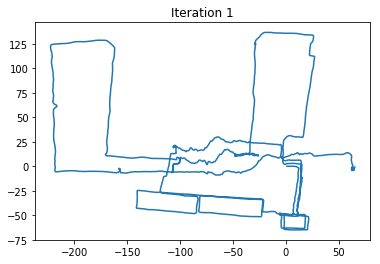
\includegraphics[width=0.4\textwidth]{4-1_by_deleji_1.png}
\end{figure}

\begin{figure}[h!]
  \centering
  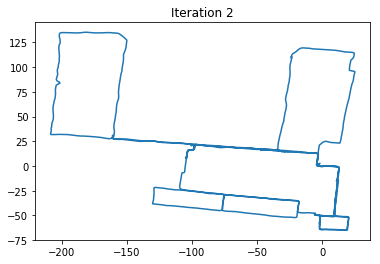
\includegraphics[width=0.4\textwidth]{4-2_by_deleji_2.png}
\end{figure}

\begin{figure}[h!]
  \centering
  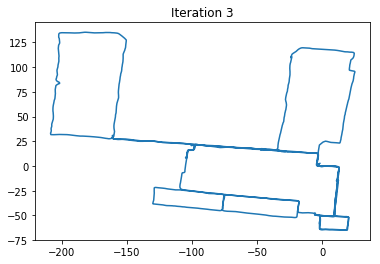
\includegraphics[width=0.4\textwidth]{4-3_by_deleji_3.png}
\end{figure}

One can see that the trajectories which regarded as different paths are restored.

\newpage

\begin{thebibliography}{99}
  \bibitem{tutorail} G. Grisetti, R. Kummerle, C. Stachniss, and W. Burgard,
    "A tutorial on graph-based SLAM",
    IEEE Intelligent Transportation Systems Magazine,
    2010.
  \bibitem{deleji} GitHub - deleji/graph-slam: 一个二维平面的激光图优化例子,
  \url{https://github.com/deleji/graph-slam}
  \bibitem{udacity} Udacity - Artificial Intelligence for Robotics: Implementing SLAM,
  \url{https://www.udacity.com/course/artificial-intelligence-for-robotics--cs373}
\end{thebibliography}

\end{document}
